\documentclass[10pt,letterpaper]{article}
\usepackage[utf8]{inputenc}
\usepackage{graphicx}
\usepackage{caption}
\usepackage{subcaption}
\author{Michael D. Brothers}
\title{Homework 5}
\begin{document}

%{\centering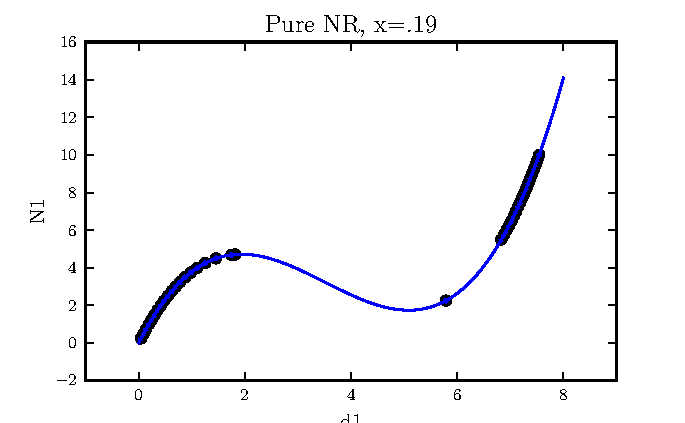
\includegraphics[width=1\textwidth]{pure_nr_x19.pdf}}
\section{Plots: exact solution}

\begin{figure}[!tbh]
  \begin{subfigure}[b]{.6\textwidth}
    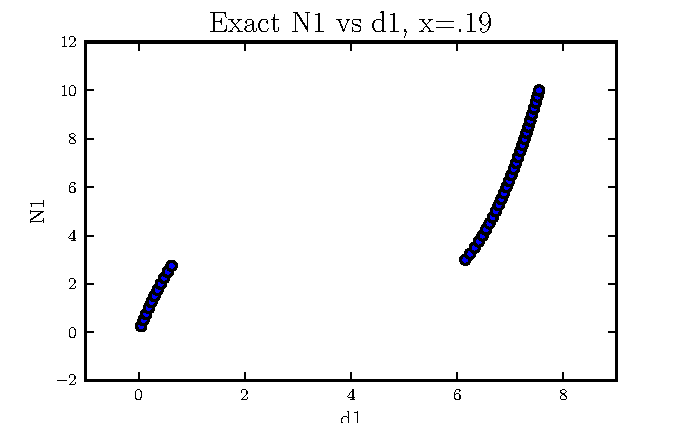
\includegraphics[width=\textwidth]{exact_x19.pdf}
    \caption{}
    \label{fig1:label:a}
  \end{subfigure}
  \hfill
  \begin{subfigure}[b]{.6\textwidth}
    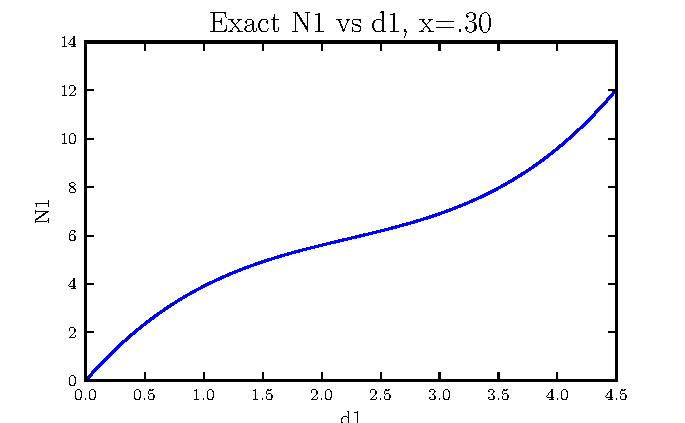
\includegraphics[width=\textwidth]{exact_x30.pdf}
    \caption{}
    \label{fig1:label:b}
  \end{subfigure}
  \caption{Exact solution curves, assuming d1=d2.}
\end{figure}

Exact solution curve, assuming d1=d2. There is reversal in slope seen in~\ref{fig1:label:a}. This feature is hinted at qualitatively but not identically expressed in ~\ref{fig1:label:b}. Overall the numerical methods handled $x=.19$ worse than $x=.30$ most likely due to the way a near zero slope with cause a naive Newton algorithm to guess a very large iterate.


\section{Plots: pure Newton}
\begin{figure}[!tbh]
  \begin{subfigure}[b]{.6\textwidth}
    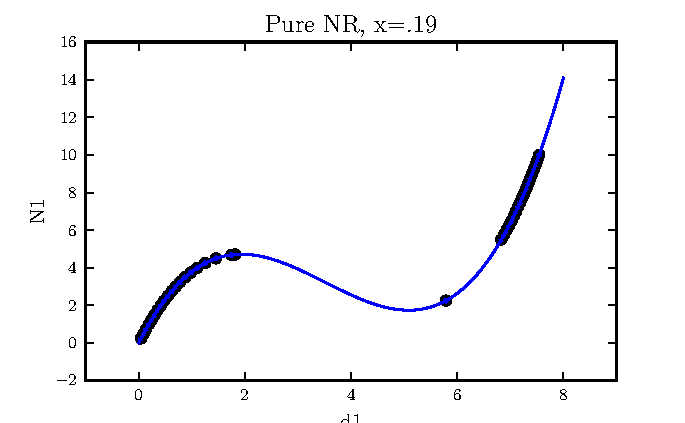
\includegraphics[width=1\textwidth]{pure_nr_x19.pdf}
    \caption{}
    \label{fig2:label:a}
  \end{subfigure}
  \hfill
  \begin{subfigure}[b]{.6\textwidth}
    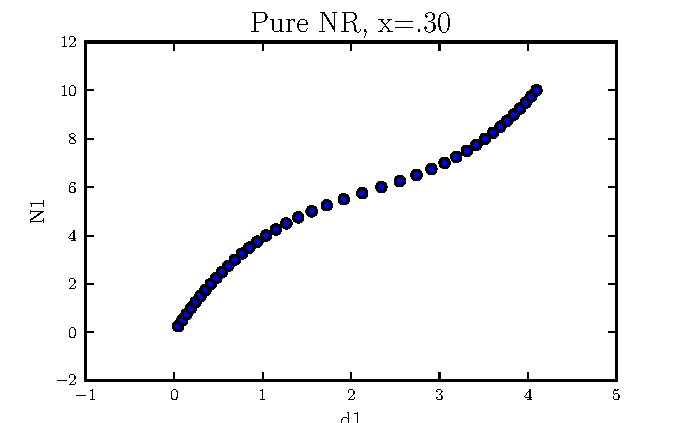
\includegraphics[width=1\textwidth]{pure_nr_x30.pdf}
    \caption{}
    \label{fig2:label:b}
  \end{subfigure}
  \hfill
    \begin{subfigure}[b]{.6\textwidth}
    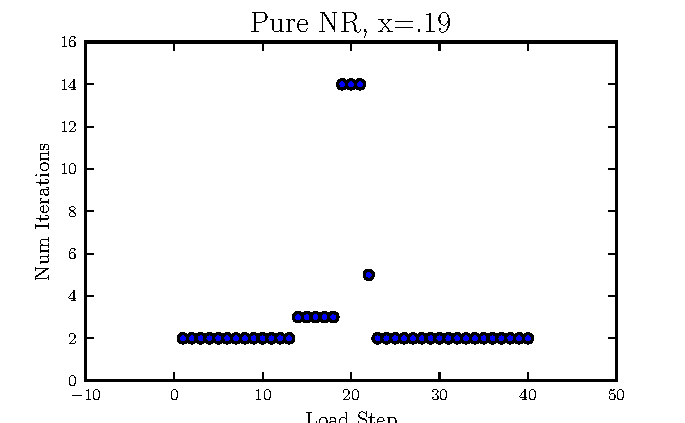
\includegraphics[width=1\textwidth]{pure_nr_x19_conv.pdf}
    \caption{}
    \label{fig2:label:c}
  \end{subfigure}
  \hfill
  \begin{subfigure}[b]{.6\textwidth}
    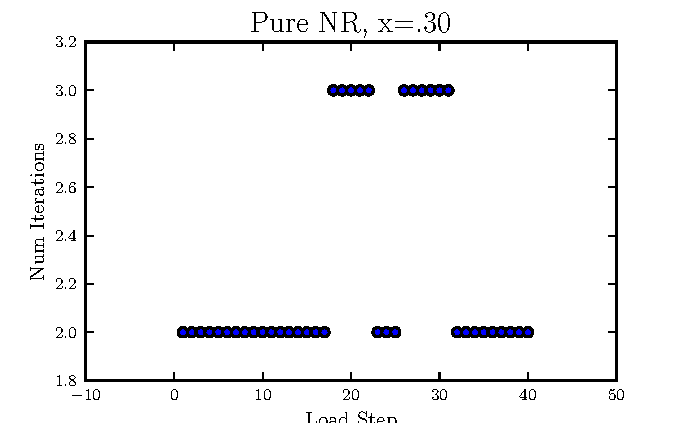
\includegraphics[width=1\textwidth]{pure_nr_x30_conv.pdf}
    \caption{}
    \label{fig2:label:d}
  \end{subfigure}
  \caption{Numerical solution curve, NR method. The method converged to approximate solutions for all loadsteps for the case that $x=.30$.
}
\end{figure}

Numerical solution curve, NR method. Looking at~\ref{fig2:label:c} the pure Newton Raphson method failed to converge after $18$ loadsteps in that case that $x=.19$. The solution saved for these loadsteps contained NaN such that they were not plotted. NaN could indicate floating point overflow such as from an iterate computed from a near singular tangent stiffness matrix as would be expected in the camel hump shaped region the solution curve progressed to before convergence ceased. It appears that convergence was recovered for the higher load values, this is because the sign of the slope is positive and stable for d1 greater than about 6. This is because a cubic polynomial like the analytic solution curve is not periodic and contains only two sign reversals in the firsts derivative. Therefore, even if a wildly inaccurate iterate brings the initial displacement guess to a d1 value much higher than the true value, since the true value lays within the slope stable region the next iterate is very accurate such that we see convergence in only 5 to 2 iterations after the solution curve was derailed so to speak~\ref{fig2:label:c}. 
The method converged to approximate solutions for all loadsteps for the case that $x=.30$.


\section{Plots: modified Newton}
\begin{figure}[!tbh]
  \begin{subfigure}[b]{.6\textwidth}
    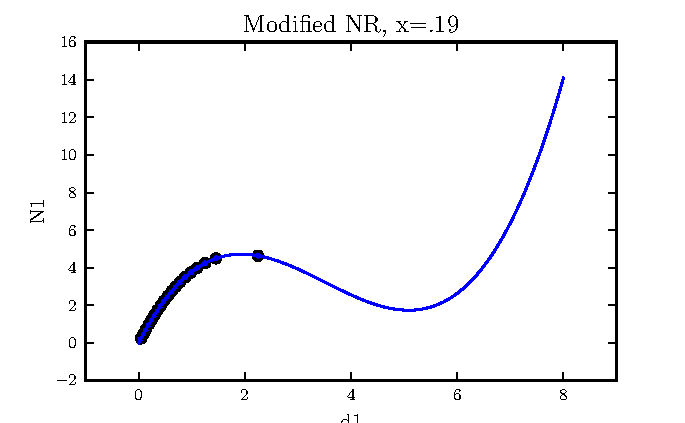
\includegraphics[width=\textwidth]{moded_nr_x19.pdf}
    \caption{}
    \label{fig3:label:a}
  \end{subfigure}
  \hfill
  \begin{subfigure}[b]{.6\textwidth}
    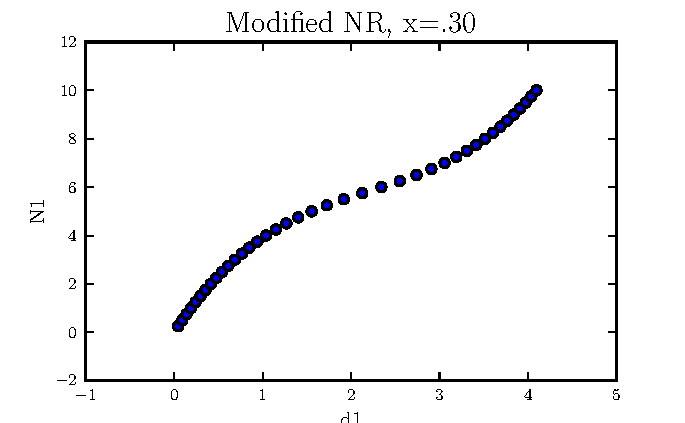
\includegraphics[width=\textwidth]{moded_nr_x30.pdf}
    \caption{}
    \label{fig3:label:b}
  \end{subfigure}
  \hfill
    \begin{subfigure}[b]{.6\textwidth}
    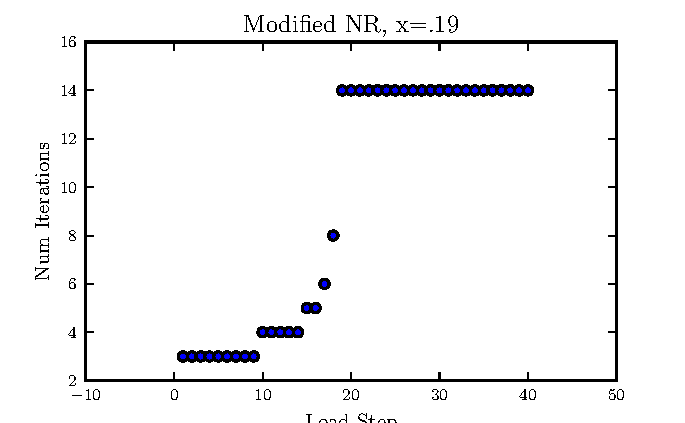
\includegraphics[width=\textwidth]{moded_nr_x19_conv.pdf}
    \caption{}
    \label{fig3:label:c}
  \end{subfigure}
  \hfill
  \begin{subfigure}[b]{.6\textwidth}
    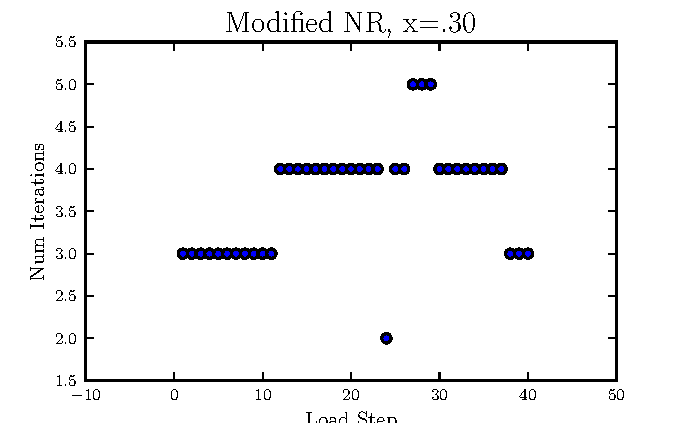
\includegraphics[width=\textwidth]{moded_nr_x30_conv.pdf}
    \caption{}
    \label{fig3:label:d}
  \end{subfigure}
  \caption{Numerical solution curves, modified NR method.}
\end{figure}

Numerical solution curve, modified NR method. Looking at~\ref{fig3:label:c} the modified Newton Raphson method failed to converge after $18$ loadsteps in that case that $x=.19$. Unlike for the pure Newton method in which the tangent stiffness matrix is rebuilt for every inner loop iteration, the modified method never reconnected with the solution curve at higher loads. This suggests that even if erroneous iterates in the slope sign stable regions were achieved, the cubic nature of the polynomial solution curve meant that an initial linear approximation to the slope did a poor job tracking the solution curve's behavior such that these initial bad guesses could be starting points for restored convergence. The method converged to approximate solutions for all loadsteps for the case that $x=.30$, however more iterations were needed than as in the pure Newton case.


\begin{figure}[!tbh]
  \begin{subfigure}[b]{.6\textwidth}
    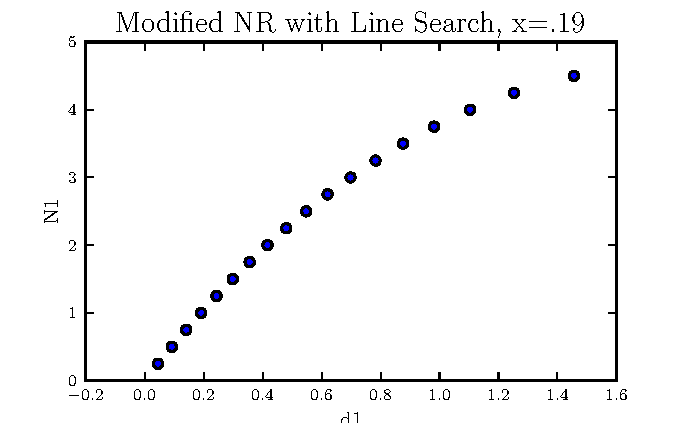
\includegraphics[width=\textwidth]{moded_nr_wls_x19.pdf}
    \caption{}
    \label{fig4:label:a}
  \end{subfigure}
  \hfill
  \begin{subfigure}[b]{.6\textwidth}
    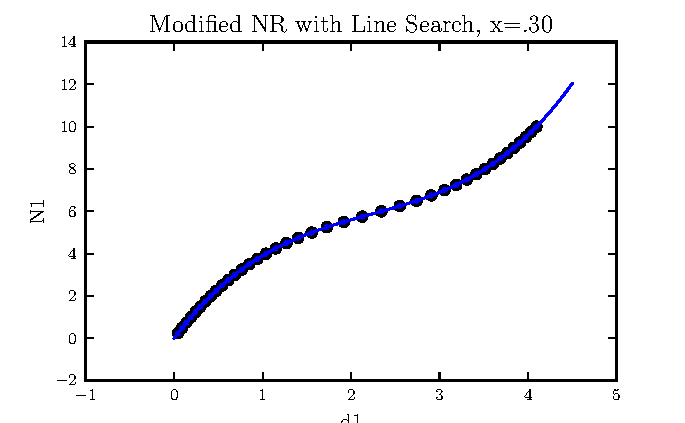
\includegraphics[width=\textwidth]{moded_nr_wls_x30.pdf}
    \caption{}
    \label{fig4:label:b}
  \end{subfigure}
  \hfill
    \begin{subfigure}[b]{.6\textwidth}
    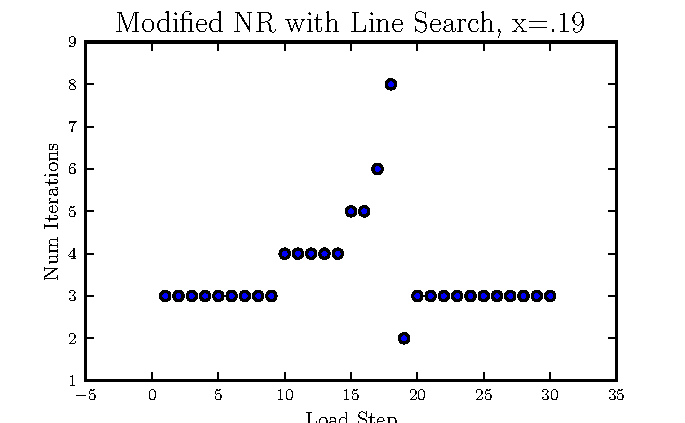
\includegraphics[width=\textwidth]{moded_nr_wls_x19_conv.pdf}
    \caption{}
    \label{fig4:label:c}
  \end{subfigure}
  \hfill
  \begin{subfigure}[b]{.6\textwidth}
    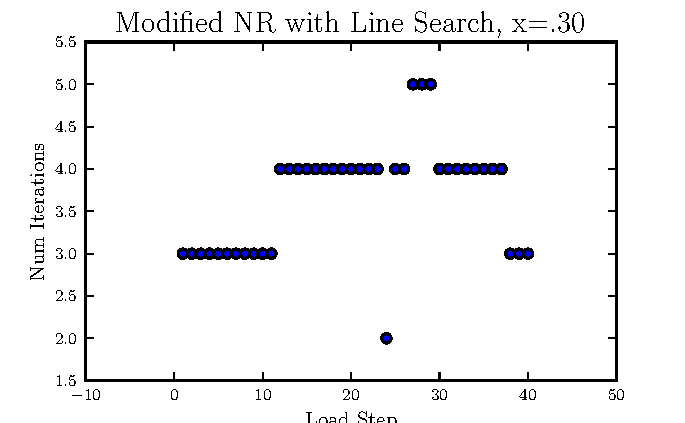
\includegraphics[width=\textwidth]{moded_nr_wls_x30_conv.pdf}
    \caption{}
    \label{fig4:label:d}
  \end{subfigure}
    \caption{Numerical solution curves, modified NR method with line search.}
\end{figure}

Numerical solution curve, modified NR method with line search. Looking at~\ref{fig4:label:c} the modified Newton Raphson method with line search failed to converge after $18$ loadsteps in that case that $x=.19$. Similarly to the pure Newton method, the solution curve was rejoined for higher loads. This is a robustness not seen in the standard modified Newton method. The method converged to approximate solutions for all loadsteps for the case that $x=.30$. In all cases convergence required at least the number of iterations required of the pure Newton method, but no more than were needed for the standard modified Newton method. It would also bear mentioning that although the number of iterations needed for convergence exceeded the number for the pure Newton method, the individual iterations for the modified Newton method with line search are less expensive since they do not entail the reconstruction of the tangent stiffness matrix.


\section{Plots: BFGS}
\begin{figure}[!tbh]
  \begin{subfigure}[b]{.6\textwidth}
    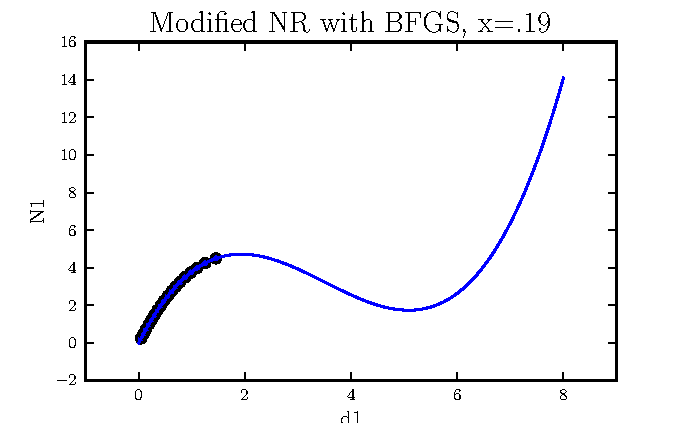
\includegraphics[width=\textwidth]{moded_nr_bfgs_x19.pdf}
    \caption{}
    \label{fig5:label:a}
  \end{subfigure}
  \hfill
  \begin{subfigure}[b]{.6\textwidth}
    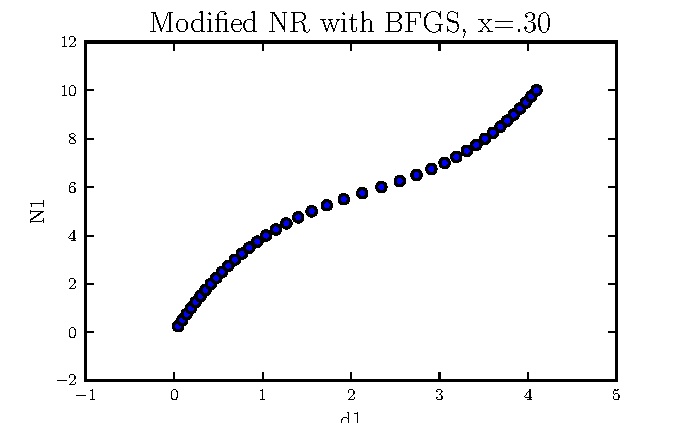
\includegraphics[width=\textwidth]{moded_nr_bfgs_x30.pdf}
    \caption{}
    \label{fig5:label:b}
  \end{subfigure}
  \hfill
    \begin{subfigure}[b]{.6\textwidth}
    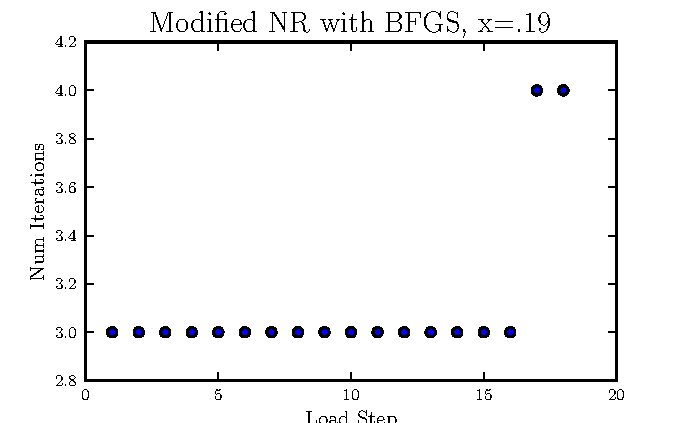
\includegraphics[width=\textwidth]{moded_nr_bfgs_x19_conv.pdf}
    \caption{}
    \label{fig5:label:c}
  \end{subfigure}
  \hfill
  \begin{subfigure}[b]{.6\textwidth}
    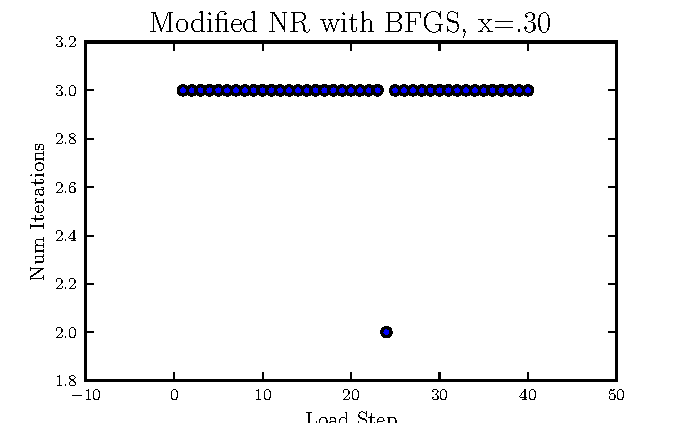
\includegraphics[width=\textwidth]{moded_nr_bfgs_x30_conv.pdf}
    \caption{}
    \label{fig5:label:d}
  \end{subfigure}
    \caption{Numerical solution curve, modified NR method with BFGS.}
\end{figure}

Numerical solution curve, modified NR method with BFGS. Looking at~\ref{fig5:label:c} the modified Newton Raphson method with BFGS failed to converge after $18$ loadsteps in that case that $x=.19$. This method showed an equally poor ability to track the solution curve as the modified Newton method, however, when convergence did occur, it was usually with fewer iterations than needed by the modified Newton method. Although, surely it is more expensive to compute the BFGS updates than to do nothing as in standard modified Newton. The method converged to approximate solutions for all loadsteps for the case that $x=.30$.


\begin{figure}[!tbh]
  \begin{subfigure}[b]{.6\textwidth}
    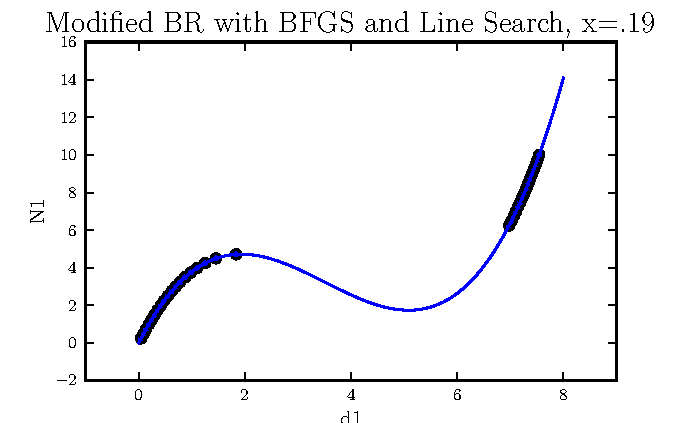
\includegraphics[width=\textwidth]{moded_nr_bfgs_wls_x19.pdf}
    \caption{}
    \label{fig6:label:a}
  \end{subfigure}
  \hfill
  \begin{subfigure}[b]{.6\textwidth}
    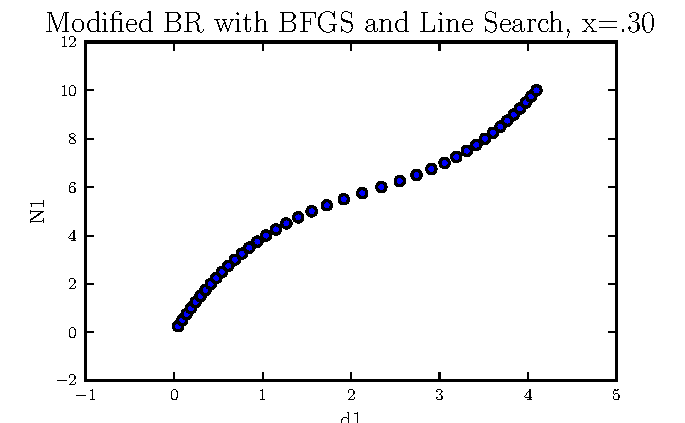
\includegraphics[width=\textwidth]{moded_nr_bfgs_wls_x30.pdf}
    \caption{}
    \label{fig6:label:b}
  \end{subfigure}
  \hfill
    \begin{subfigure}[b]{.6\textwidth}
    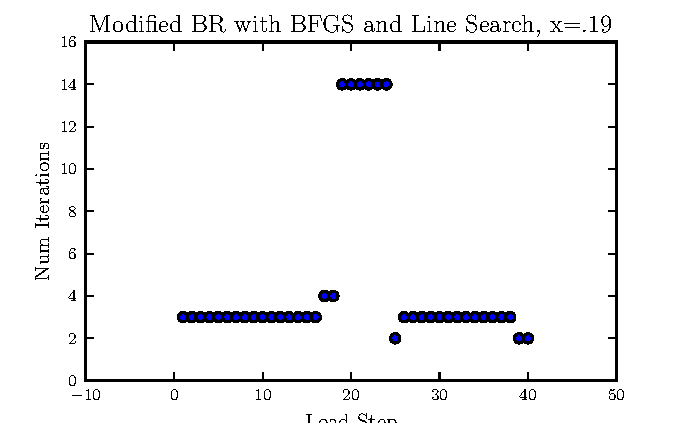
\includegraphics[width=\textwidth]{moded_nr_bfgs_wls_x19_conv.pdf}
    \caption{}
    \label{fig6:label:c}
  \end{subfigure}
  \hfill
  \begin{subfigure}[b]{.6\textwidth}
    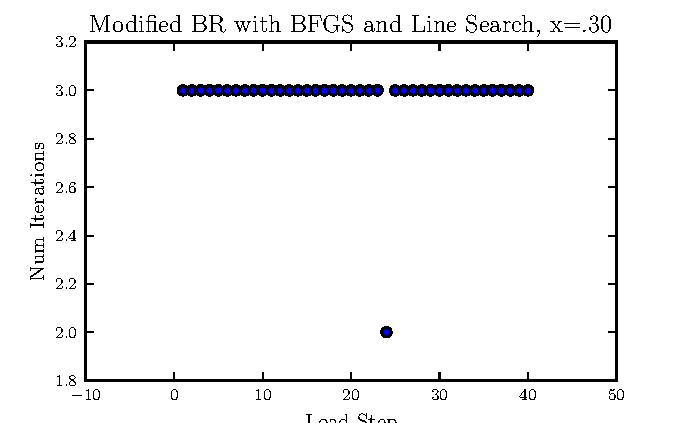
\includegraphics[width=\textwidth]{moded_nr_bfgs_wls_x30_conv.pdf}
    \caption{}
    \label{fig6:label:d}
  \end{subfigure}
    \caption{Numerical solution curve, modified NR method with BFGS and line search.}
\end{figure}

Numerical solution curve, modified NR method with BFGS and line search. Looking at~\ref{fig6:label:c} the modified Newton Raphson method with BFGS and line search failed to converge after $18$ loadsteps in that case that $x=.19$. The modified BFGS method recovers the ability to rejoin the solution curve at higher loads. This is a quality shared with the pure Newton method as well as the modified Newton method with line search. This method decidedly has a superior convergence rate to the modified Newton and standard BFGS algorithms, but in a general setting this might be outweighed by the additional work it needs to do per iteration when compared with those other methods. However, the per iteration computational intensity is still less than that of the pure Newton method while from a qualitative standpoint, the same solution curve information can be computed, especially the rejoining of the solution curve at higher load levels. The rejoining itself suggests that the BFGS updates are able to convey sufficient information such that even though the tangent stiffness matrix is not being rebuilt, the cubic behavior of the solution curve could be tracked after divergence brought the iterate to a distant erroneous value. The method converged to approximate solutions for all loadsteps for the case that $x=.30$.

\pagebreak
\section{Data tables: $x=.19$, solution curve}
\begin{figure}
\begin{tabular}{rrrrrrrrrr}
\hline
    pure d &    pure N &   modified d &   modified N &   modified wls d &   modified wls N &      BFGS d &    BFGS N &   BFGS wls d &   BFGS wls N \\
\hline
 0.0453748 &  0.249999 &    0.0453743 &     0.249996 &        0.0453743 &         0.249996 &   0.045375  &   0.25    &    0.045375  &      0.25    \\
 0.0923015 &  0.499999 &    0.0923008 &     0.499995 &        0.0923008 &         0.499995 &   0.0923017 &   0.5     &    0.0923017 &      0.5     \\
 0.140926  &  0.749999 &    0.140925  &     0.749994 &        0.140925  &         0.749994 &   0.140927  &   0.75    &    0.140927  &      0.75    \\
 0.191419  &  0.999998 &    0.191418  &     0.999993 &        0.191418  &         0.999993 &   0.19142   &   1       &    0.19142   &      1       \\
 0.243981  &  1.25     &    0.243979  &     1.24999  &        0.243979  &         1.24999  &   0.243981  &   1.25    &    0.243981  &      1.25    \\
 0.298847  &  1.5      &    0.298846  &     1.49999  &        0.298846  &         1.49999  &   0.298848  &   1.5     &    0.298848  &      1.5     \\
 0.356305  &  1.75     &    0.356303  &     1.74999  &        0.356303  &         1.74999  &   0.356306  &   1.75    &    0.356306  &      1.75    \\
 0.416702  &  2        &    0.416699  &     1.99998  &        0.416699  &         1.99998  &   0.416703  &   2       &    0.416703  &      2       \\
 0.480468  &  2.24999  &    0.480464  &     2.24998  &        0.480464  &         2.24998  &   0.480469  &   2.25    &    0.480469  &      2.25    \\
 0.548149  &  2.49999  &    0.548151  &     2.5      &        0.548151  &         2.5      &   0.548151  &   2.5     &    0.548151  &      2.5     \\
 0.620452  &  2.74999  &    0.620454  &     2.75     &        0.620454  &         2.75     &   0.620455  &   2.75    &    0.620455  &      2.75    \\
 0.698318  &  2.99999  &    0.698321  &     3        &        0.698321  &         3        &   0.698322  &   3       &    0.698322  &      3       \\
 0.783052  &  3.24998  &    0.783058  &     3.24999  &        0.783058  &         3.24999  &   0.78306   &   3.25    &    0.78306   &      3.25    \\
 0.876565  &  3.5      &    0.87656   &     3.49999  &        0.87656   &         3.49999  &   0.876564  &   3.5     &    0.876564  &      3.5     \\
 0.981786  &  3.75     &    0.981785  &     3.75     &        0.981785  &         3.75     &   0.981784  &   3.75    &    0.981784  &      3.75    \\
 1.10377   &  4        &    1.10377   &     3.99999  &        1.10377   &         3.99999  &   1.10377   &   3.99999 &    1.10377   &      3.99999 \\
 1.25263   &  4.25     &    1.25262   &     4.24999  &        1.25262   &         4.24999  &   1.25263   &   4.25    &    1.25263   &      4.25    \\
 1.45581   &  4.5      &    1.4558    &     4.49999  &        1.4558    &         4.49999  &   1.45581   &   4.5     &    1.45581   &      4.5     \\
 1.81673   &  4.71194  &    2.24726   &     4.64062  &        1.70966   &         4.67769  & nan         & nan       &    1.83648   &      4.7158  \\
 1.74815   &  4.69264  &  nan         &   nan        &        1.70966   &         4.67769  & nan         & nan       &    1.83648   &      4.7158  \\
 5.78901   &  2.25413  &  nan         &   nan        &        1.70966   &         4.67769  & nan         & nan       &    1.83648   &      4.7158  \\
 6.83277   &  5.5      &  nan         &   nan        &        1.70966   &         4.67769  & nan         & nan       &    1.83648   &      4.7158  \\
 6.88301   &  5.75     &  nan         &   nan        &        1.70966   &         4.67769  & nan         & nan       &    1.83648   &      4.7158  \\
 6.93141   &  6        &  nan         &   nan        &        1.70966   &         4.67769  & nan         & nan       &    6.98129   &      6.26725 \\
 6.97813   &  6.25     &  nan         &   nan        &        1.70966   &         4.67769  & nan         & nan       &    6.97813   &      6.25    \\
 7.02331   &  6.5      &  nan         &   nan        &        1.70966   &         4.67769  & nan         & nan       &    7.02331   &      6.5     \\
 7.06709   &  6.75     &  nan         &   nan        &        1.70966   &         4.67769  & nan         & nan       &    7.06709   &      6.75    \\
 7.10956   &  7        &  nan         &   nan        &        7.14272   &         7.20034  & nan         & nan       &    7.10956   &      7       \\
 7.15083   &  7.25     &  nan         &   nan        &        7.15083   &         7.25     & nan         & nan       &    7.15083   &      7.25    \\
 7.19098   &  7.5      &  nan         &   nan        &        7.19098   &         7.5      & nan         & nan       &    7.19098   &      7.5     \\
 7.23008   &  7.75     &  nan         &   nan        &        7.23008   &         7.75     & nan         & nan       &    7.23008   &      7.75    \\
 7.26821   &  8        &  nan         &   nan        &        7.26821   &         8        & nan         & nan       &    7.26821   &      8       \\
 7.30542   &  8.25     &  nan         &   nan        &        7.30542   &         8.25     & nan         & nan       &    7.30542   &      8.25    \\
 7.34177   &  8.5      &  nan         &   nan        &        7.34177   &         8.5      & nan         & nan       &    7.34177   &      8.5     \\
 7.37731   &  8.75     &  nan         &   nan        &        7.37731   &         8.75     & nan         & nan       &    7.37731   &      8.75    \\
 7.41208   &  9        &  nan         &   nan        &        7.41208   &         9        & nan         & nan       &    7.41208   &      9       \\
 7.44612   &  9.25     &  nan         &   nan        &        7.44612   &         9.25     & nan         & nan       &    7.44612   &      9.25    \\
 7.47948   &  9.5      &  nan         &   nan        &        7.47948   &         9.5      & nan         & nan       &    7.47948   &      9.5     \\
 7.51219   &  9.75     &  nan         &   nan        &        7.51219   &         9.75     & nan         & nan       &    7.51219   &      9.74998 \\
 7.54428   & 10        &  nan         &   nan        &        7.54428   &        10        & nan         & nan       &    7.54427   &      9.99998 \\
\hline
\end{tabular}
\caption{Solution approximations, $x=.19$}
\end{figure}
\begin{figure}
\begin{tabular}{rrrrrrrrrr}
\hline
    pure d &    pure N &   modified d &   modified N &   modified wls d &   modified wls N &    BFGS d &   BFGS N &   BFGS wls d &   BFGS wls N \\
\hline
 0.0453729 &  0.249999 &    0.0453724 &     0.249996 &        0.0453724 &         0.249996 & 0.0453731 &  0.25    &    0.0453731 &      0.25    \\
 0.092285  &  0.499999 &    0.0922844 &     0.499995 &        0.0922844 &         0.499995 & 0.0922852 &  0.5     &    0.0922852 &      0.5     \\
 0.140865  &  0.749999 &    0.140865  &     0.749995 &        0.140865  &         0.749995 & 0.140866  &  0.75    &    0.140866  &      0.75    \\
 0.191261  &  0.999998 &    0.19126   &     0.999994 &        0.19126   &         0.999994 & 0.191261  &  1       &    0.191261  &      1       \\
 0.243639  &  1.25     &    0.243638  &     1.24999  &        0.243638  &         1.24999  & 0.24364   &  1.25    &    0.24364   &      1.25    \\
 0.298193  &  1.5      &    0.298192  &     1.49999  &        0.298192  &         1.49999  & 0.298194  &  1.5     &    0.298194  &      1.5     \\
 0.355146  &  1.75     &    0.355144  &     1.74999  &        0.355144  &         1.74999  & 0.355146  &  1.75    &    0.355146  &      1.75    \\
 0.414757  &  2        &    0.414755  &     1.99999  &        0.414755  &         1.99999  & 0.414758  &  2       &    0.414758  &      2       \\
 0.477332  &  2.25     &    0.47733   &     2.24999  &        0.47733   &         2.24999  & 0.477333  &  2.25    &    0.477333  &      2.25    \\
 0.543234  &  2.5      &    0.54323   &     2.49998  &        0.54323   &         2.49998  & 0.543235  &  2.5     &    0.543235  &      2.5     \\
 0.612893  &  2.74999  &    0.612889  &     2.74998  &        0.612889  &         2.74998  & 0.612895  &  2.75    &    0.612895  &      2.75    \\
 0.686835  &  2.99999  &    0.686836  &     3        &        0.686836  &         3        & 0.686837  &  3       &    0.686837  &      3       \\
 0.765695  &  3.24999  &    0.765698  &     3.25     &        0.765698  &         3.25     & 0.765698  &  3.25    &    0.765698  &      3.25    \\
 0.850264  &  3.49999  &    0.850267  &     3.5      &        0.850267  &         3.5      & 0.850267  &  3.5     &    0.850267  &      3.5     \\
 0.941523  &  3.74999  &    0.941527  &     3.75     &        0.941527  &         3.75     & 0.941528  &  3.75    &    0.941528  &      3.75    \\
 1.04071   &  3.99998  &    1.04072   &     3.99999  &        1.04072   &         3.99999  & 1.04072   &  4       &    1.04072   &      4       \\
 1.14941   &  4.24998  &    1.14942   &     4.24999  &        1.14942   &         4.24999  & 1.14942   &  4.25    &    1.14942   &      4.25    \\
 1.26964   &  4.5      &    1.26963   &     4.49999  &        1.26963   &         4.49999  & 1.26964   &  4.5     &    1.26964   &      4.5     \\
 1.40386   &  4.75     &    1.40385   &     4.74998  &        1.40385   &         4.74998  & 1.40386   &  4.75    &    1.40386   &      4.75    \\
 1.55503   &  5        &    1.55501   &     4.99998  &        1.55501   &         4.99998  & 1.55502   &  5       &    1.55502   &      5       \\
 1.72599   &  5.25     &    1.72597   &     5.24998  &        1.72597   &         5.24998  & 1.72599   &  5.25    &    1.72599   &      5.25    \\
 1.91793   &  5.5      &    1.91792   &     5.49999  &        1.91792   &         5.49999  & 1.91793   &  5.5     &    1.91793   &      5.5     \\
 2.12718   &  5.74999  &    2.12718   &     5.75     &        2.12718   &         5.75     & 2.12718   &  5.75    &    2.12718   &      5.75    \\
 2.34285   &  6        &    2.34285   &     6        &        2.34285   &         6        & 2.34286   &  6.00001 &    2.34286   &      6.00001 \\
 2.55048   &  6.25001  &    2.55047   &     6.25     &        2.55047   &         6.25     & 2.55047   &  6.25    &    2.55047   &      6.25    \\
 2.73997   &  6.5      &    2.73995   &     6.49998  &        2.73995   &         6.49998  & 2.73996   &  6.5     &    2.73996   &      6.5     \\
 2.90845   &  6.75     &    2.90845   &     6.75     &        2.90845   &         6.75     & 2.90845   &  6.75    &    2.90845   &      6.75    \\
 3.05743   &  7        &    3.05743   &     7        &        3.05743   &         7        & 3.05743   &  7       &    3.05743   &      7       \\
 3.18984   &  7.25     &    3.18984   &     7.25     &        3.18984   &         7.25     & 3.18983   &  7.25    &    3.18983   &      7.25    \\
 3.30855   &  7.5      &    3.30855   &     7.49998  &        3.30855   &         7.49998  & 3.30855   &  7.5     &    3.30855   &      7.5     \\
 3.41603   &  7.75     &    3.41602   &     7.74999  &        3.41602   &         7.74999  & 3.41603   &  7.75    &    3.41603   &      7.75    \\
 3.51421   &  8.00002  &    3.51419   &     7.99999  &        3.51419   &         7.99999  & 3.5142    &  8       &    3.5142    &      8       \\
 3.60461   &  8.25002  &    3.6046    &     8.24999  &        3.6046    &         8.24999  & 3.6046    &  8.25    &    3.6046    &      8.25    \\
 3.68844   &  8.50001  &    3.68844   &     8.5      &        3.68844   &         8.5      & 3.68844   &  8.5     &    3.68844   &      8.5     \\
 3.76668   &  8.75001  &    3.76668   &     8.75     &        3.76668   &         8.75     & 3.76668   &  8.75    &    3.76668   &      8.75    \\
 3.84008   &  9.00001  &    3.84008   &     9        &        3.84008   &         9        & 3.84008   &  9       &    3.84008   &      9       \\
 3.90926   &  9.25001  &    3.90926   &     9.25     &        3.90926   &         9.25     & 3.90926   &  9.25    &    3.90926   &      9.25    \\
 3.97475   &  9.5      &    3.97475   &     9.50002  &        3.97475   &         9.50002  & 3.97475   &  9.5     &    3.97475   &      9.5     \\
 4.03695   &  9.75     &    4.03695   &     9.75002  &        4.03695   &         9.75002  & 4.03695   &  9.75    &    4.03695   &      9.75    \\
 4.09623   & 10        &    4.09623   &    10        &        4.09623   &        10        & 4.09623   & 10       &    4.09623   &     10       \\
\hline
\end{tabular}
\caption{Solution approximations, $x=.30$}
\end{figure}
\begin{figure}
\begin{tabular}{llllllllllllllllllllllllllllllllllllllll}
\hline
                       &                       &                       &                       &                       &                       &                       &                       &                       &                       &                       &                       &                       &                       &                       &                       &                       &                       &                            &                            &                            &                            &                            &                            &                            &                            &                            &                            &                            &                            &                            &                            &                            &                            &                            & pure                       & modified                   & modified wls               & BFGS                       & BFGS wls                   \\
\hline
 [ 2.  3.  3.  3.  3.] & [ 2.  3.  3.  3.  3.] & [ 2.  3.  3.  3.  3.] & [ 2.  3.  3.  3.  3.] & [ 2.  3.  3.  3.  3.] & [ 2.  3.  3.  3.  3.] & [ 2.  3.  3.  3.  3.] & [ 2.  3.  3.  3.  3.] & [ 2.  3.  3.  3.  3.] & [ 2.  4.  4.  3.  3.] & [ 2.  4.  4.  3.  3.] & [ 2.  4.  4.  3.  3.] & [ 2.  4.  4.  3.  3.] & [ 3.  4.  4.  3.  3.] & [ 3.  5.  5.  3.  3.] & [ 3.  5.  5.  3.  3.] & [ 3.  6.  6.  4.  4.] & [ 3.  8.  8.  4.  4.] & [ 14.  14.  14.  14.  14.] & [ 14.  14.  14.  14.  14.] & [ 14.  14.  14.  14.  14.] & [  5.  14.  14.  14.  14.] & [  2.  14.  14.  14.  14.] & [  2.  14.  14.  14.  14.] & [  2.  14.  14.  14.   2.] & [  2.  14.  14.  14.   3.] & [  2.  14.  14.  14.   3.] & [  2.  14.  14.  14.   3.] & [  2.  14.   2.  14.   3.] & [  2.  14.   3.  14.   3.] & [  2.  14.   3.  14.   3.] & [  2.  14.   3.  14.   3.] & [  2.  14.   3.  14.   3.] & [  2.  14.   3.  14.   3.] & [  2.  14.   3.  14.   3.] & [  2.  14.   3.  14.   3.] & [  2.  14.   3.  14.   3.] & [  2.  14.   3.  14.   3.] & [  2.  14.   3.  14.   2.] & [  2.  14.   3.  14.   2.] \\
\hline
\end{tabular}
\caption{Number of iterations, $x=.19$}
\end{figure}
\begin{figure}
\begin{tabular}{llllllllllllllllllllllllllllllllllllllll}
\hline
                       &                       &                       &                       &                       &                       &                       &                       &                       &                       &                       &                       &                       &                       &                       &                       &                       &                       &                       &                       &                       &                       &                       &                       &                       &                       &                       &                       &                       &                       &                       &                       &                       &                       &                       & pure                  & modified              & modified wls          & BFGS                  & BFGS wls              \\
\hline
 [ 2.  3.  3.  3.  3.] & [ 2.  3.  3.  3.  3.] & [ 2.  3.  3.  3.  3.] & [ 2.  3.  3.  3.  3.] & [ 2.  3.  3.  3.  3.] & [ 2.  3.  3.  3.  3.] & [ 2.  3.  3.  3.  3.] & [ 2.  3.  3.  3.  3.] & [ 2.  3.  3.  3.  3.] & [ 2.  3.  3.  3.  3.] & [ 2.  3.  3.  3.  3.] & [ 2.  4.  4.  3.  3.] & [ 2.  4.  4.  3.  3.] & [ 2.  4.  4.  3.  3.] & [ 2.  4.  4.  3.  3.] & [ 2.  4.  4.  3.  3.] & [ 2.  4.  4.  3.  3.] & [ 3.  4.  4.  3.  3.] & [ 3.  4.  4.  3.  3.] & [ 3.  4.  4.  3.  3.] & [ 3.  4.  4.  3.  3.] & [ 3.  4.  4.  3.  3.] & [ 2.  4.  4.  3.  3.] & [ 2.  2.  2.  2.  2.] & [ 2.  4.  4.  3.  3.] & [ 3.  4.  4.  3.  3.] & [ 3.  5.  5.  3.  3.] & [ 3.  5.  5.  3.  3.] & [ 3.  5.  5.  3.  3.] & [ 3.  4.  4.  3.  3.] & [ 3.  4.  4.  3.  3.] & [ 2.  4.  4.  3.  3.] & [ 2.  4.  4.  3.  3.] & [ 2.  4.  4.  3.  3.] & [ 2.  4.  4.  3.  3.] & [ 2.  4.  4.  3.  3.] & [ 2.  4.  4.  3.  3.] & [ 2.  3.  3.  3.  3.] & [ 2.  3.  3.  3.  3.] & [ 2.  3.  3.  3.  3.] \\
\hline
\end{tabular}
\caption{Number of iterations, $x=.30$}
\end{figure}


\end{document}
